\chapter{Desenvolvimento}
  
\section{O funcionamento do termistor}
 
	O termistor é um resistor variável à temperatura, característica pela qual seu nome é inspirado (temperatura + resistor), geralmente compostos por uma liga que contém cerâmica e outros polímeros. Suas aplicações mais habituais costumam acontecer em circuitos de monitoramento e controle de temperatura ou como limitador de corrente de partida. São separados, basicamente, em duas categorias:
	\begin{itemize}
		\item NTC (Negative Temperature Coefficient): São termistores que diminuem a sua resistência à medida em que a temperatura aumenta; E
		\item PTC (Positive Temperature Coefficient): Termistores que aumentam a sua resistência diretamente com o aumento da temperatura.
	\end{itemize}
	
	\subsection{A equação de Steinhart–Hart}
	
		A curva de variação da resistência de um termistor em função de sua temperatura pode ser descrita pela equação de Steinhart–Hart\ref{eq:steinharthart} em sua forma inversa \ref{eq:steinharthartinverted}. A característica logarítmica da resposta com que a resistência varia em função da variação de temperatura (figura \ref{fig:curva_termistor}) é, em grande parte das vezes, uma das principais vantagens do seu uso, visto que pequenas variações na temperatura provocam grandes alterações na resistência, fazendo com que o sensor seja mais suscetível a detectar pequenas mudanças na temperatura.
		
		
		\begin{equation}\label{eq:steinharthart}
		\dfrac{1}{T} = a + b\ln{(R)} + c(\ln{(R)})^3
		\end{equation}
		Sendo:
		\begin{itemize}
			\item T: Temperatura em Kelvins;
			\item R: Resistência em ohms ($\Omega$);E
			\item a,b e c: Coeficientes de Steinhart–Hart, que são variáveis conforme o tipo de material e a construção do termistor.		
		\end{itemize}
		
		
		\begin{equation}\label{eq:steinharthartinverted}
			\begin{aligned} [left]
			& R = \exp{(\sqrt[3]{\beta - \dfrac{\alpha}{2}} - \sqrt[3]{\beta + \dfrac{\alpha}{2}})},
			\\
			& \alpha = \dfrac{1}{c}(a - \dfrac{1}{T}),
			\\
			& \beta = \sqrt{(\dfrac{b}{3c})^3 + (\dfrac{\alpha}{2})^2}
			\end{aligned}
		\end{equation}
	
	
		\begin{figure}[h!]
			\begin{center}
				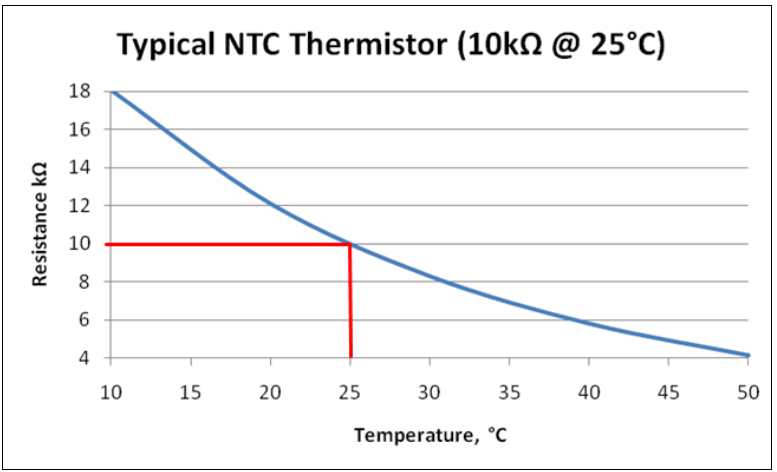
\includegraphics[width=1\linewidth]{images/curva_termistor.png}
				\caption[Curva de resposta típica em termistores NTC de 10k$\Omega$]{Curva de resposta típica em termistores NTC de 10k$\Omega$\footnotemark}
				\label{fig:curva_termistor}
			\end{center}
		\end{figure}
	
		\footnotetext{Fonte: http://www.squids.com.br/arduino/index.php/projetos-arduino/projetos-squids/basico/159-projeto-42-comparando-sensores-de-temperatura-ntc-10k-dht11-e-lm35}


	\subsection{O efeito de Autoaquecimento}

		Como toda resistência, o termistor dissipa energia elétrica na forma de calor. Portanto, ao aplicar uma corrente no sensor, é induzido um efeito de autoaquecimento. A relação da potência elétrica dissipada é dada pela equação \ref{eq:potenciaeletrica} e a relação entre potência e temperatura pode ser obtida através da equação \ref{eq:potenciatermica}. Fazendo $P_E = P_T$, é possível chegar à equação \ref{eq:temperaturacomautoaquecimento}. 
		
		\begin{equation}\label{eq:potenciaeletrica}
			P_E = I.V
		\end{equation}
		sendo:
		\begin{itemize}
			\item $P_E$: Potência elétrica dissipada;
			\item $I$: Corrente elétrica;E
			\item $V$: Tensão entre os terminais.
		\end{itemize}

		\begin{equation}\label{eq:potenciatermica}
			P_T = K(T_{(R)} - T_0)
		\end{equation}
		sendo:
		\begin{itemize}
			\item $P_T$: Potência;
			\item $K$: Fator de dissipação do termistor;
			\item $T_{(R)}$: Temperatura em função da resistência;E
			\item $T_0$: Temperatura ao redor do termistor.
		\end{itemize}
		
		\begin{equation} \label{eq:temperaturacomautoaquecimento}
			T_0 = T_{(R)} - \dfrac{V^2}{K.R}
		\end{equation}
		

\section{A evolução do circuito}
 
Valendo-se da propriedade logarítmica do termistor, uma pequena variação de temperatura ambiente ocasionada pelo processo de expiração ocasionaria uma mudança exponencial no valor da resistência. Por esse motivo, na origem do projeto, era esperada uma medição simples, obtida através da variação de tensão em um divisor resistivo composto por um termistor e uma resistência padrão(Figura: \ref{fig:divisorResistivo}). Contudo, devido alguns contratempos práticos, diversas mudanças fizeram-se necessárias. 
 

 
Uma das principais limitações para o desenvolvimento do projeto deve-se à dificuldade na aquisição dos componentes eletrônicos que, quando comprados via internet, necessitavam de um tempo para entrega relativamente alto e, para a compra realizada diretamente na loja física, existe uma limitação na variedade de lojas especializadas na cidade do Rio de Janeiro. Outra complicação relevante é referente à ausência de datasheet, que não é informado no momento da compra e torna-se impossível inferir qual é o datasheet correto apenas observando o componente, que é muito pequeno, sem qualquer informação sobre o fabricante ou o modelo. Dadas essas condições iniciais, foi construído o primeiro divisor resistivo apenas com base na informação de que o sensor adquirido tratava-se de um termistor NTC (do inglês Negative Temperature Coefficient) com resistência em temperatura ambiente de $10K\Omega$. Foi utilizada uma fonte de alimentação comercial de $12V$ e utilizado diversos valores entre $10K\Omega$ e $330\Omega$ para a resistência $R2$, contudo para nenhum valor de $R2$ era observada qualquer alteração de tensão na medida em que o ar era exalado próximo ao sensor, contrariando ao que era esperado, dado que a queda de tensão em cima do termistor deve ser variável junto à alteração na resistência.
 
\begin{figure}[h!]
	\begin{center}
 		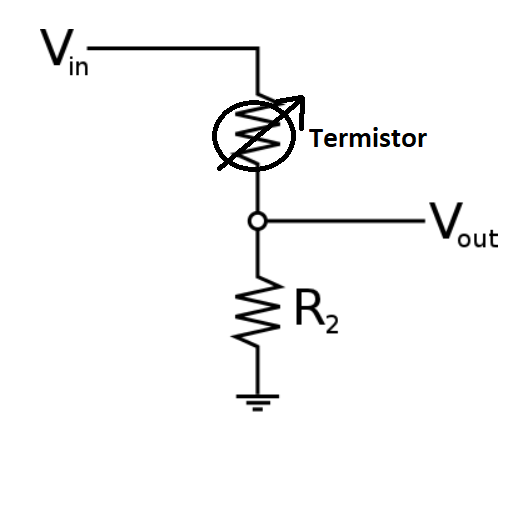
\includegraphics[width=0.5\linewidth]{images/divisor_resistivo.png}
 		\caption{Divisor Resistivo}
 		\label{fig:divisorResistivo}
 	\end{center}
\end{figure}
 
A lei de resfriamento de newton (\ref{eq:resfriamento}) indica que a taxa com que um corpo perde calor é proporcional à diferença de temperatura entre o corpo e o meio  no qual ele se encontra. Valendo-se desse princípio, nota-se que uma baixa diferença de temperatura resultaria em um maior tempo de resposta do sensor. Portanto, para contornar o problema obtido, o circuito foi ajustado para utilizar a propriedade de autoaquecimento do termistor (\ref{eq:autoAquecimento}). 
 
  
\begin{equation} \label{eq:resfriamento}
	\dfrac{dQ}{dt} = h.A.(T(t) - T_{env}) = h.A \Delta T(t)	
\end{equation}
Onde:
\begin{itemize}[label=]
	\item $Q$: Energia térmica
	\item $t$: Tempo
	\item $h$: Coeficiente de transferência de calor
	\item $A$: Área de transferência de calor
	\item $T$: Temperatura do objeto
	\item $T_{env}$: Temperatura do ambiente
\end{itemize}
 
\begin{equation} \label{eq:autoAquecimento}
	T_0 = T(R) - \dfrac{V^2}{KR}
\end{equation}
Onde:
\begin{itemize}[label=]
	\item $T_0$: Temperatura do meio
 	\item $T(R)$: Temperatura do termistor em função de sua resistência
 	\item $V$: Diferença de potencial entre os terminais do termistor
 	\item $K$: Fator de dissipação do termistor
 	\item $R$: Resistência
\end{itemize}
 
 
 
Ao aplicar uma alta corrente no sensor, é induzido então um aumento na temperatura deste. Em decorrência desse aumento, é possível observar uma maior diferença de temperatura entre o sensor e o fluxo de ar e, por conseguinte, uma maior taxa para transferência de calor e um menor tempo de resposta por parte do termistor. Contudo, para atingir uma faixa de temperatura sensível, capaz de gerar uma resposta visível ao expor o sensor à respiração, o circuito necessita de uma tensão elevada, acima das entregues por fontes comerciais padrão, que costumam variar entre $5V$ e $12V$, gerando a necessidade de projetar um retificador de tensão capaz de converter a tensão de corrente alternada entregue pela rede elétrica residencial em uma tensão contínua alta o suficiente para fornecer ao termistor a corrente demandada.
 
Realizando testes de bancada, com um gerador de tensão variando de $0V$ à $30V$ e uma resistência de $330\Omega$ em série com o termistor, foi possível atingir uma temperatura sensível ao sopro, entretanto, ao aplicar uma tensão em torno de $22V$, o sensor demorava um tempo considerável para aquecer novamente, tornando-o inviável para medir o comportamento respiratório dada a frequência do sopro em uma respiração normal. Aumentando a tensão para $28V$, já era possível observar uma atenuação considerável na queda constante da temperatura dado que o termistor era capaz de se aquecer mais rápido. O problema gerado por esse aumento de tensão deve-se ao fato de que, quanto maior é a corrente, maior é o autoaquecimento e, quanto maior a temperatura, menor é a resistência, gerando um aumento ainda maior na corrente passante que, por sua vez, aumenta ainda mais a temperatura até que o sensor atingia um patamar no qual queimava, caso não houvesse nenhum sopro forçando a temperatura a diminuir. 
 
Se por um lado, o aumento da tensão era importante para que a temperatura não decaísse constantemente ao iniciar a medição respiratória, por outro, o sistema precisava ser protegido para que a corrente não atingisse um determinado patamar que danificasse o componente. O ajuste mais simples para regular a corrente em um componente costuma ser adicionar uma resistência em série, diminuindo a corrente por uma mera consequência da lei de ohm (\ref{eq:leideohm}). Contudo, por se tratar de uma resistência variável, a tensão necessária para o aquecimento do termistor em seu estado inicial era maior que a tensão necessária para mantê-lo abaixo de um patamar seguro após a diminuição de sua resistência pelo efeito do autoaquecimento. Foi pensado então em um circuito de controle não linear (Figura: \ref{fig:circuitoRealimentado}), que, em teoria, forneceria uma alta tensão para o termistor até que sua resistência variasse e a corrente passante atingisse um patamar determinado. 
  
\begin{equation} \label{eq:leideohm}
	V = R.I
\end{equation}
Onde:
\begin{itemize}[label=]
  	\item $V$: Tensão
  	\item $R$: Resistência
  	\item $I$: Corrente
\end{itemize}

\begin{figure}[h!]
	\begin{center}
		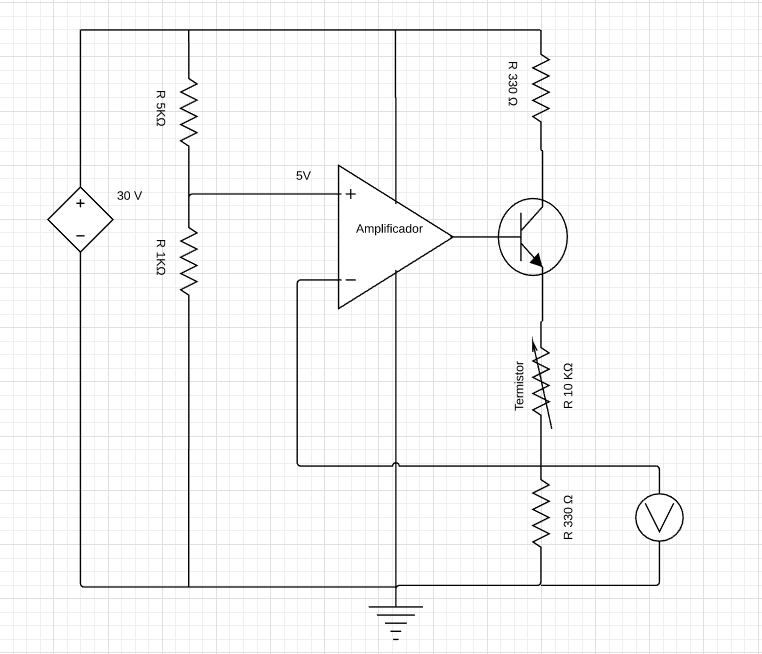
\includegraphics[width=1\linewidth]{images/Circuito_de_controle.png}
		\caption{Circuito de Controle}
		\label{fig:circuitoRealimentado}
	\end{center}
\end{figure}

O comportamento esperado para o circuito de controle seria o seguinte: O amplificador operacional iria ajustar a tensão de saída na tentativa de igualar as tensões nos dois terminais de entrada, sendo assim, no momento inicial, quando a tensão no terminal de entrada negativo é igual a zero e a do terminal positivo é igual a $5V$, o amplificador aumenta sua saída fazendo com que o transistor entre em saturação e conduza uma corrente no emissor praticamente igual à de referência no coletor, na medida em que a resistência do termistor diminui pelo efeito de autoaquecimento, a tensão de saída aumenta até que esta se iguale à do terminal positivo, ao atingir esse patamar, o transistor saí da zona de saturação e o sistema trabalha pra manter a tensão de saída constante. No momento em que o sensor entra em contato com o fluxo de ar, a resistência do termistor aumenta, diminuindo a tensão na saída e estimulando o sistema de controle a saturar o transistor e induzir o efeito do autoaquecimento no sensor. Após quantizar a tensão da saída através de um microcontrolador, foi possível traçar o gráfico da figura \ref{fig:RespostaCircuitoRealimentado}, no qual aparece nítida a resposta do sistema ao submeter o sensor a um fluxo de ar. Entretanto, ao expor o sensor a um período prolongado de exposição à respiração humana, foi possível observar que o efeito do resfriamento contínuo continuava a ser reproduzido (gráfico da figura \ref{fig:RespostaCircuitoRealimentadoLongoPrazo}).


\begin{figure}[h!]
	\begin{center}
		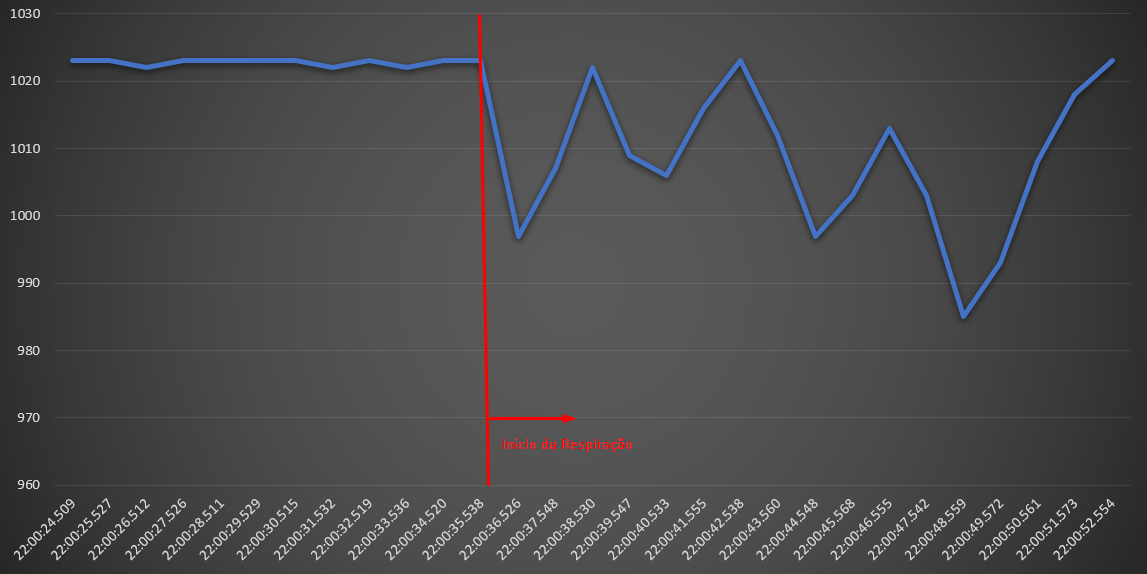
\includegraphics[width=1\linewidth]{images/RespostaCircuitoRealimentado.png}
		\caption{Resposta em curto prazo circuito realimentado (Tempo no eixo horizontal e valor de tensão quantizado no eixo vertical)}
		\label{fig:RespostaCircuitoRealimentado}
	\end{center}
\end{figure}

\begin{figure}[h!]
	\begin{center}
		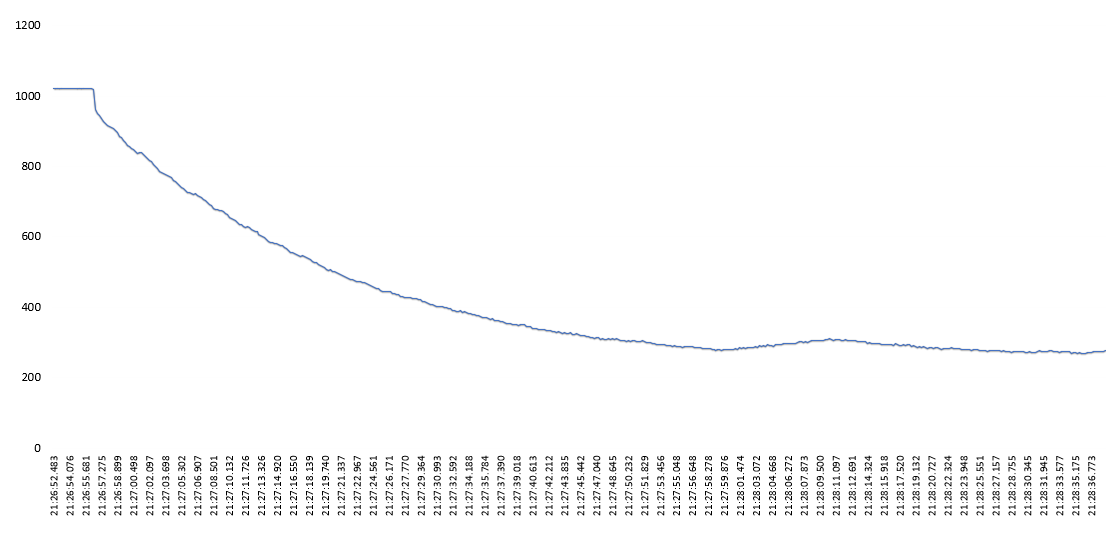
\includegraphics[width=1\linewidth]{images/DecaimentoRespiracaoMascara.png}
		\caption{Resposta de longo prazo circuito realimentado (Tempo no eixo horizontal e valor de tensão quantizado no eixo vertical)}
		\label{fig:RespostaCircuitoRealimentadoLongoPrazo}
	\end{center}
\end{figure}


%\section{A fonte de tensão}
 
 